% =============================================================
%  main.tex -- Override-Locked NIDS (Elsevier preprint)
%  Compiler  : pdfLaTeX
%  Class     : elsarticle (preprint, author-year citations)
%  HOW TO USE:
%    1. Run  python paper/generate_figures.py  (once)
%    2. Upload main.tex, refs.bib, figures/ to Overleaf
%    3. Compile: pdfLaTeX -> BibTeX -> pdfLaTeX -> pdfLaTeX
% =============================================================
\documentclass[preprint,12pt,authoryear]{elsarticle}

% -- Encoding & fonts ------------------------------------------
\usepackage[utf8]{inputenc}
\usepackage[T1]{fontenc}
\usepackage{microtype}

% -- Mathematics -----------------------------------------------
\usepackage{amsmath,amssymb,amsthm}

% -- Tables ----------------------------------------------------
\usepackage{booktabs}
\usepackage{multirow}
\usepackage{tabularx}
\usepackage{array}

% -- Figures ---------------------------------------------------
\usepackage{graphicx}
\usepackage{subcaption}
\usepackage{float}
\graphicspath{{figures/}}

% -- TikZ (pipeline & flow diagrams) --------------------------
\usepackage{tikz}
\usetikzlibrary{shapes.geometric,arrows.meta,positioning,
                fit,backgrounds,shadows.blur}
\usepackage{pgfplots}
\pgfplotsset{compat=1.18}

% -- Hyperlinks & cross-references ----------------------------
\usepackage[hidelinks]{hyperref}
\usepackage[capitalise,nameinlink]{cleveref}

% -- Algorithms -----------------------------------------------
\usepackage[ruled,vlined,linesnumbered]{algorithm2e}

% -- Misc typography ------------------------------------------
\usepackage{xcolor}
\usepackage{siunitx}
\DeclareSIUnit{\ms}{ms}           % millisecond shorthand
\usepackage{url}
\usepackage{lineno}               % remove before camera-ready

% -- Theorem environments -------------------------------------
\newtheorem{definition}{Definition}

% -- Colours --------------------------------------------------
\definecolor{pass1col}{RGB}{52,138,189}
\definecolor{pass2col}{RGB}{214,80,68}
\definecolor{graybox}{RGB}{245,245,245}

% -- Journal --------------------------------------------------
\journal{Computers \& Security}   % change to target journal

% =============================================================
\begin{document}
\linenumbers   % remove before camera-ready

\begin{frontmatter}

\title{Context-Aware Counterfactual Explanations for\\
       Real-Time Network Intrusion Detection:\\
       A Multi-Pass Override Decomposition Framework}

% TODO: fill in affiliation; add co-authors if applicable
\author[a]{Mohamed Benjari}
\ead{your.email@institution.edu}

\affiliation[a]{%
  organization={Department of Computer Science},
  addressline={},
  city={},
  postcode={},
  country={}}

% -- Abstract -------------------------------------------------
\begin{abstract}
Anomaly-based network intrusion detection systems (NIDS) achieve high detection
rates but produce decisions that security analysts cannot interpret, verify, or
act upon---a condition that drives alert fatigue and erodes operational trust.
The problem is particularly acute when enforcement decisions are locked by
policy overrides: existing counterfactual explanation methods, designed for
continuous feature perturbation, cannot explain why a decision is structurally
irreversible.
This paper presents a context-aware KitNET IDS pipeline that addresses this gap
through a four-pass, latency-bounded counterfactual (CF) engine with a dedicated
override decomposition pass.
Evaluated on 99{,}999 packets from a real Mirai IoT botnet capture, the system
detects 9{,}685 anomalies (9.7\%) and produces actionable explanations for
97.6\% of them.
A structural finding emerges from the CF pass distribution: 87.2\% of anomalies
require Pass~2 (override decomposition) to explain their enforcement decision,
while only 10.5\% are resolved by single-feature perturbation.
This result reveals that for botnet-class traffic, the dominant explanation
bottleneck lies in the classification rule---not in the anomaly threshold.
The CF engine achieves a mean latency of \SI{0.06}{\ms} per packet
(p95: \SI{0.08}{\ms}) with zero timeouts across all four budget modes
(\textsc{strict} \SI{2}{\ms}, \textsc{normal} \SI{10}{\ms},
\textsc{relaxed} \SI{50}{\ms}, \textsc{batch} unlimited), confirming
real-time feasibility.
A human-feedback learning module reduces the false positive rate from 2.77\% to
0.00\% within one feedback round using multiplicative weight updates, while a
sliding-window drift detector identifies concept drift in all three synthetic
transition scenarios tested.
We document a vulnerability to sustained adversarial feedback that establishes
no clean baseline, motivating mitigations discussed in \cref{sec:disc_poison}.
These findings motivate the pass decomposition architecture as a design
consideration for IDS operating on botnet-class traffic, particularly where
attack-type classification overrides are a structural component of the enforcement
pipeline.
Evaluated on a second dataset (UNSW-NB15, 82{,}332 flows, 9 attack categories),
the autoencoder anomaly detector achieves AUC~0.81 with 97.1\% precision at a
strict 99th-percentile threshold (System~A), rising to 84.3\% recall when the
decision layer is applied (System~B).
A LIME and SHAP comparison confirms the structural limitation: 100\% of LIME
score/risk perturbations fail to change the enforcement action for override-locked
packets, versus 52\% for non-override-locked packets.
\end{abstract}

\begin{keyword}
network intrusion detection \sep counterfactual explanation \sep
explainable AI \sep KitNET \sep anomaly detection \sep
feedback learning \sep concept drift \sep override decomposition
\end{keyword}

\end{frontmatter}

% =============================================================
\section{Introduction}
\label{sec:intro}
% =============================================================

Security operations centres (SOCs) are under sustained pressure from alert
fatigue. A 2022 survey by the Ponemon Institute found that the average security
team receives more than 11{,}000 alerts per day, of which roughly 45\% are
false positives~\citep{Ponemon2022}. The burden falls disproportionately on
anomaly-based NIDS, where the absence of explicit decision logic makes
individual alerts difficult to triage, verify, or refute. Analysts confronted
with an opaque anomaly score have no principled mechanism to determine whether
the alert represents a genuine threat, a benign statistical deviation, or a
tuning artefact---a problem identified by Sommer and Paxson as the
foundational operationalisation challenge of anomaly
detection~\citep{Sommer2010}.

Explainable AI (XAI) methods have been proposed as a solution. Techniques such
as LIME~\citep{Ribeiro2016} and SHAP~\citep{Lundberg2017} generate post-hoc
feature attributions that can, in principle, tell an analyst which input
features contributed most to an anomaly score. Counterfactual
explanations~\citep{Wachter2018} go further: they answer the actionable
question, ``What would have had to be different for this packet to have been
allowed?''---giving the analyst a concrete, hypothetical handle on the decision
boundary. Both families of methods have been applied to NIDS
settings~\citep{Antwarg2021,Wang2022}, demonstrating that feature-level
explanations can reduce analyst response time and improve decision confidence.

However, a critical gap exists in the current literature: none of these methods
account for \emph{policy-level override locking}. Modern hybrid
NIDS---systems that combine an anomaly detector with a rule-based attack
classifier and a structured decision layer---produce enforcement decisions that
cannot be reversed by any perturbation of the anomaly score alone. When a
packet is classified as ``Mirai C2 Communication'' and the decision layer issues
a \textsc{block} via a hard override, no reduction in the KitNET RMSE score will
change that outcome. The correct counterfactual explanation is structural: ``This
packet would have been \textsc{allowed} if the attack classification rule had not
fired''---but this explanation requires decomposing the override logic, not
perturbing a continuous feature. Existing CF methods, which assume a
differentiable or at least monotone scoring function, cannot produce this class
of explanation.

This paper makes four primary contributions:

\begin{enumerate}
\item \textbf{A multi-pass counterfactual engine with override decomposition
  (Pass~2)} that explains policy-locked decisions by stripping the attack
  classification override and computing the hypothetical action under the
  baseline risk model, then identifying the minimum score or risk change that
  would further shift that action. Pass~2 is, to our knowledge, the first
  published CF method specifically designed for the override layer of hybrid
  NIDS.

\item \textbf{A structural finding on the dominance of override-locked
  decisions}: evaluated on 9{,}685 detected anomalies from a Mirai IoT botnet
  capture, 87.2\% (8{,}440 packets) require Pass~2 to receive a meaningful
  explanation, while only 10.5\% (1{,}014 packets) are explained by
  single-feature perturbation (Pass~1). This result holds because 86.0\% of
  anomalies are classified as Mirai C2 Communication---a botnet-specific
  traffic pattern whose enforcement decision is structurally override-locked.

\item \textbf{Real-time CF feasibility at a mean latency of \SI{0.06}{\ms}
  per packet}: across four budget modes with designed limits of \SI{2}{\ms},
  \SI{10}{\ms}, \SI{50}{\ms}, and no limit, the CF engine records zero timeouts
  and a p95 latency of \SI{0.08}{\ms}, confirming that explanation generation
  does not constrain packet-level processing.

\item \textbf{A feedback learning module that eliminates false positives within
  one round}: using multiplicative weight updates (MWU), the weight-only
  configuration reduces the false positive rate from 2.77\% to 0.00\% at
  Round~1 with F1~= 0.9991 (81{,}999 evaluable rows). A convergence speed
  ablation reveals that threshold-only adaptation, while it also eliminates
  FP (at Round~7), does so at the cost of catastrophic false-negative inflation
  (97.7\% FN by Round~10), making weight-only the operationally stable choice.

\item \textbf{Empirical validation of the structural limitation via LIME and
  SHAP comparison}: a surrogate random forest (5-fold F1~=~0.9992) trained on
  (score, risk, $t$, override\_locked) features shows that LIME score/risk
  perturbations fail to change the enforcement action for 100\% of
  override-locked anomalies, versus 52\% for non-override-locked anomalies.
  SHAP attributes 48.3\% of importance to the override\_locked feature for
  override-locked packets, confirming that attribution alone cannot replace
  structural counterfactual decomposition.

\item \textbf{Cross-dataset evaluation on UNSW-NB15}: applied to 82{,}332
  flows across 9 attack categories (Generic, Exploits, Fuzzers, DoS,
  Reconnaissance, and others), the MLP autoencoder achieves AUC~=~0.81.
  Adding the decision layer (System~B) raises recall from 29.3\% to 84.3\%,
  demonstrating that the decision-layer integration generalises beyond
  Mirai-class traffic.
\end{enumerate}

The remainder of this paper is organised as follows. \Cref{sec:background}
surveys related work. \Cref{sec:architecture} describes the system architecture.
\Cref{sec:evaluation} presents experimental results. \Cref{sec:discussion}
discusses implications and limitations. \Cref{sec:limitations} enumerates
disclosed limitations. \Cref{sec:conclusion} concludes with directions for
future work.

% =============================================================
\section{Background and Related Work}
\label{sec:background}
% =============================================================

\subsection{Anomaly-Based Network Intrusion Detection}
\label{subsec:anomaly_nids}

Anomaly-based NIDS identify malicious traffic by comparing observed behaviour
against a baseline model of normality, flagging deviations as anomalies. This
approach generalises to novel attacks---unlike signature-based systems, which
require prior knowledge of attack patterns---but introduces a fundamental
challenge: without an explicit attack model, detected anomalies carry no
semantic content, and analysts receive only a numeric score.

KitNET~\citep{Mirsky2018}, introduced by Mirsky et al.\ in 2018, addresses
scalability in anomaly-based NIDS through an online, unsupervised ensemble of
lightweight autoencoders. Each autoencoder operates on a correlated subset of
features produced by the AfterImage statistics module, which computes five
running statistics (mean, standard deviation, radius, magnitude, and
correlation) for each of up to five network channel abstractions (MAC-IP, IP,
socket, host-port, and host-host). The ensemble output---an RMSE reconstruction
error---serves as the anomaly score. KitNET requires no labelled data and
processes packets at line rate, making it attractive for deployment in
resource-constrained environments. However, KitNET's reconstruction error is a
continuous scalar with no semantic grounding: an RMSE of 0.35 conveys no more
information to an analyst than a Z-score without a distribution reference.

Buczak and Guven~\citep{Buczak2016} survey machine learning methods for cyber
security intrusion detection, noting that the dominant challenge across all
anomaly detection paradigms is the generation of actionable alerts---alerts that
give an analyst sufficient context to make a confident triage decision.

\subsection{Counterfactual Explanations}
\label{subsec:cf_background}

Wachter, Mittelstadt, and Russell~\citep{Wachter2018} established counterfactual
explanations as a principled approach to algorithmic
transparency~\citep{Molnar2022}, framing the problem as finding the minimum
perturbation to an input that changes a model's output. Their formulation is
model-agnostic and optimises for sparsity (few changed features) and proximity
(small magnitude of change)---properties that directly translate to the analyst
context: a sparse, proximate CF tells an analyst precisely which signal drove
the decision and how far from the boundary the packet currently lies.

DICE (Diverse Counterfactual Explanations)~\citep{Mothilal2020} extends this by
generating a set of diverse CFs rather than a single nearest counterfactual.
LEMNA~\citep{Guo2018} specifically targets deep learning-based security
applications, approximating the local decision boundary with a mixture model
and generating feature-level explanations through perturbation sampling.
DICE, LEMNA, and the model-agnostic CF framework of Karimi et
al.~\citep{Karimi2020} all assume a differentiable or continuously approximable
scoring function. None can address override-locked decisions that arise in
hybrid NIDS where a rule-based classifier determines the enforcement action
independently of the anomaly score.

\subsection{XAI for Security}
\label{subsec:xai_security}

Lundberg and Lee~\citep{Lundberg2017} (SHAP) demonstrated that additive feature
attributions can be computed efficiently for tree-based and neural classifiers;
several works have applied SHAP to NIDS feature
attribution~\citep{Antwarg2021}. LIME~\citep{Ribeiro2016} has similarly been
applied to IDS models in the UNSW-NB15 and NSL-KDD evaluation
settings~\citep{Wang2022}, identifying which network statistics---packet rate,
byte count, connection duration---contribute most to anomaly classifications.

However, these attributions are fundamentally retrospective: they explain why a
score was high, not what would have had to change for the decision to be
different. In operational settings where analysts must prioritise and respond to
alerts in real time, the counterfactual framing is significantly more
actionable~\citep{Wachter2018}. Furthermore, neither SHAP nor LIME account for
the decision layer between the anomaly score and the enforcement action: in a
hybrid NIDS, a SHAP attribution on the KitNET score does not explain why that
score produced a \textsc{block} rather than an \textsc{alert}.

\subsection{Adaptive IDS and Feedback Learning}
\label{subsec:adaptive_ids}

Online learning in NIDS addresses the challenge of concept drift---the
progressive degradation of a classifier trained on a static snapshot of normal
traffic as new protocols, services, and attack patterns emerge. Bifet and
Gavalda~\citep{Bifet2007} introduced ADWIN (Adaptive Windowing), a statistically
grounded algorithm for detecting and adapting to change in data streams.
Gama et al.~\citep{Gama2004} proposed the Drift Detection Method (DDM), which
monitors the error rate of a classifier and signals drift when the error rate
rises significantly above the baseline observed during a low-error period.

Human-in-the-loop approaches introduce analyst feedback as an additional
learning signal. Active learning systems for IDS~\citep{Miller2020} ask analysts
to label uncertain examples, prioritising the most informative queries to
maximise labelling efficiency. The system described in this paper extends this
paradigm: rather than querying the analyst, it processes unsolicited feedback
(false positive and true positive markings) and uses that signal both to adjust
per-context feature weights and to detect concept drift from the pattern of
analyst corrections.

\subsection{Research Gap}
\label{subsec:gap}

The combination of counterfactual explanation, hybrid NIDS decision layers, and
human feedback has not previously been addressed in an integrated framework.
Existing CF methods cannot explain override-locked decisions; existing
XAI-for-IDS methods do not account for policy layers; and adaptive IDS systems
that incorporate human feedback have not modelled the analyst's false positive
signal as a drift indicator. This paper addresses all three gaps.

% =============================================================
\section{System Architecture}
\label{sec:architecture}
% =============================================================

\subsection{Overview}
\label{subsec:overview}

The system processes raw PCAP network captures through a linear pipeline:
feature extraction and anomaly scoring (KitNET), risk amplification (risk
engine), threshold-based detection (adaptive threshold), attack classification
(rule engine), structured enforcement (decision layer), multi-module explanation
(explainability quad), counterfactual generation, and feedback learning.
\Cref{fig:pipeline} illustrates the pipeline.

% -- Figure 1: System Pipeline ---------------------------------
\begin{figure*}[t]
\centering
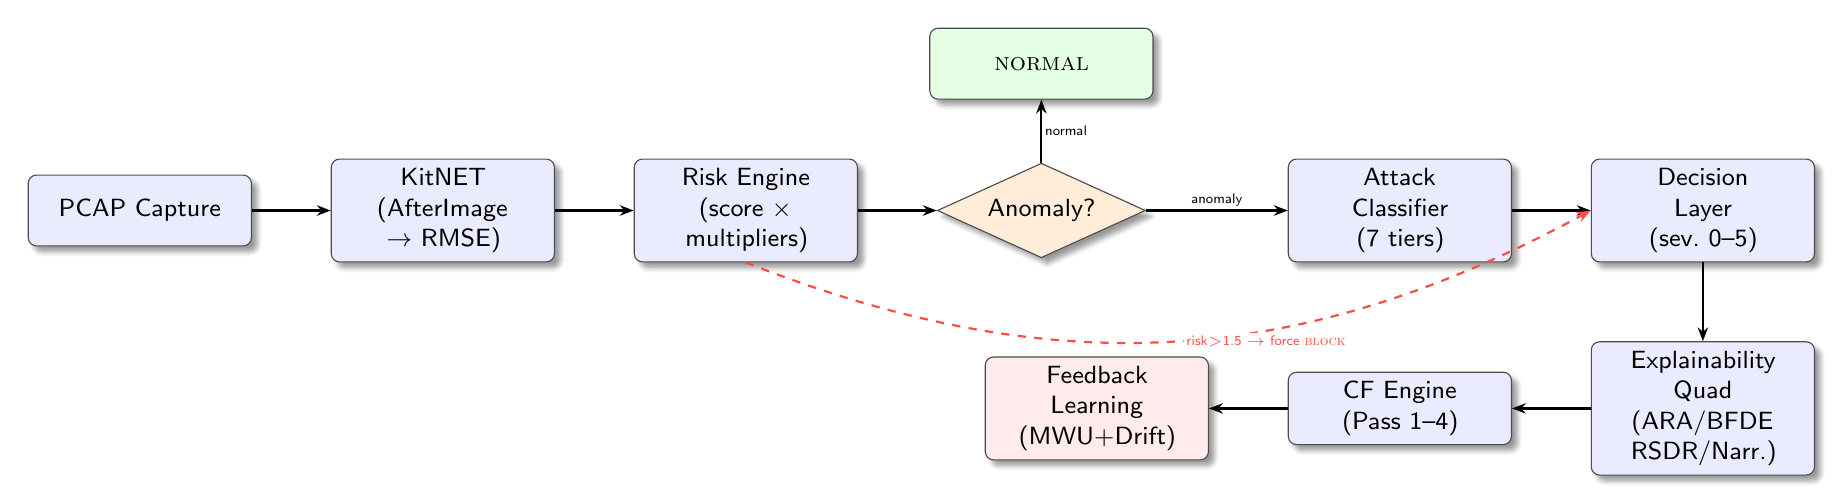
\begin{tikzpicture}[
  node distance = 6mm and 10mm,
  every node/.style = {font=\small\sffamily},
  block/.style = {rectangle, rounded corners=3pt, draw=black!70, fill=blue!8,
    text width=26mm, align=center, minimum height=9mm,
    blur shadow={shadow blur steps=5}},
  decision/.style = {
    diamond, aspect=2.2, draw=black!70, fill=orange!15,
    text width=18mm, align=center, inner sep=1pt,
    blur shadow={shadow blur steps=5}},
  green_block/.style = {block, fill=green!10},
  red_block/.style   = {block, fill=red!8},
  arr/.style = {-{Stealth[length=5pt]}, thick},
  lbl/.style = {font=\tiny\sffamily, fill=white, inner sep=1pt}
]

\node[block]                         (pcap)   {PCAP Capture};
\node[block,  right=of pcap]         (kit)    {KitNET\\(AfterImage\\$\to$ RMSE)};
\node[block,  right=of kit]          (risk)   {Risk Engine\\(score $\times$\\multipliers)};
\node[decision, right=of risk]       (thresh) {Anomaly?};
\node[green_block, above=8mm of thresh] (normal) {\textsc{normal}};
\node[block,  right=18mm of thresh]  (atk)    {Attack\\Classifier\\(7 tiers)};
\node[block,  right=of atk]          (dec)    {Decision\\Layer\\(sev.\ 0--5)};
\node[block,  below=10mm of dec]     (expl)   {Explainability\\Quad\\(ARA/BFDE\\RSDR/Narr.)};
\node[block,  left=of expl]          (cf)     {CF Engine\\(Pass 1--4)};
\node[red_block, left=of cf]         (fb)     {Feedback\\Learning\\(MWU+Drift)};

\draw[arr] (pcap) -- (kit);
\draw[arr] (kit)  -- (risk);
\draw[arr] (risk) -- (thresh);
\draw[arr] (thresh) -- node[lbl,above]{anomaly} (atk);
\draw[arr] (thresh) -- node[lbl,right]{normal}  (normal);
\draw[arr] (atk)  -- (dec);
\draw[arr] (dec)  -- (expl);
\draw[arr] (expl) -- (cf);
\draw[arr] (cf)   -- (fb);
\draw[arr,dashed,red!70] (risk.south)
  to[bend right=25]
  node[lbl,right,xshift=1mm]{\tiny risk$>$1.5 $\to$ force \textsc{block}}
  (dec.west);
\end{tikzpicture}
\caption{System pipeline. PCAP packets flow through KitNET anomaly scoring,
  risk amplification, and adaptive threshold detection. Detected anomalies are
  classified by a seven-tier rule engine and routed through the decision layer
  to the explainability quad and CF engine. The dashed red arrow indicates the
  hard override path (risk $>$ 1.5 bypasses the threshold and forces
  \textsc{block}). Analyst feedback updates feature weights and the detection
  threshold via the feedback learning module.}
\label{fig:pipeline}
\end{figure*}

\subsection{Detection Layer}
\label{subsec:detection}

\paragraph{KitNET and AfterImage.}
KitNET~\citep{Mirsky2018} processes each packet through the AfterImage feature
extractor, which maintains exponentially decaying statistics over five network
channel abstractions. The extractor produces a feature vector of up to 100
dimensions representing running mean, standard deviation, radius, magnitude, and
Pearson correlation for each channel at multiple time-decay constants
($\lambda = 5$, $3$, $1$). KitNET trains an ensemble of lightweight autoencoders
on the first $\text{FMgrace} + \text{ADgrace}$ packets (20{,}000 in this
deployment, split equally), then enters detection mode where each packet's
reconstruction RMSE is the anomaly signal.

\paragraph{Risk Engine.}
The raw RMSE score is amplified by a composite risk engine applying
context-dependent multipliers: an endpoint weight drawn from a traffic profile,
a rate multiplier active when packet frequency exceeds 50 packets per 30-second
window, a jitter multiplier for irregular inter-arrival timing, and a packet
length signal. This multi-signal formulation ensures that identical KitNET scores
produce different risk levels depending on the operational context of the
traffic.

\paragraph{Adaptive Threshold.}
The threshold separating \textsc{normal} from \textsc{anomaly} is maintained by
an online adaptive mechanism using Welford's algorithm over a sliding window of
250 samples. Three operational modes are supported: \texttt{high\_security}
($k = 1.6$), \texttt{balanced} ($k = 1.8$), and \texttt{low\_noise} ($k = 2.5$),
where $k$ is the number of standard deviations above the mean that defines the
detection boundary. A maximum cap of 2.5 prevents unbounded drift toward false
negatives. The experimental deployment used \texttt{low\_noise} (\textsc{normal})
mode.

\subsection{Classification Layer}
\label{subsec:classification}

Anomaly-detected packets are passed to a seven-tier rule-based attack classifier
that assigns a semantic attack label based on KitNET score, risk, context
features, and packet-level signals. Tiers are ordered from most-specific to
least-specific: (1) Mirai C2/loader port traffic, (2) stealth/low-and-slow
intrusion, (3) C2 beaconing, (4) data exfiltration, (5) port scanning, (6)
DoS/flood, and (7) a catch-all ``Suspicious Activity'' tier.

\subsection{Decision Layer}
\label{subsec:decision}

\begin{definition}[Override-Locked Decision]
\label{def:override_locked}
Let $f\colon S \times R \times T \times Q \to A$ denote the hybrid NIDS
decision function, where $S$ is the anomaly score space, $R$ the risk score
space, $T$ the set of attack-type labels (including the empty label~$\emptyset$),
$Q$ the frequency space, and $A$ the enforcement action set. Let
$\Omega\colon T \to A$ be a partial function (the \emph{override matrix})
defined on a subset $T_\Omega \subset T$. When $t \in T_\Omega$, the decision
function satisfies $f(s, r, t, q) = \Omega(t)$ for all $(s, r, q)$. A decision
$f(s, r, t, q) = a$ is \textbf{override-locked} iff $t \in T_\Omega$.
Equivalently, the action $a$ is invariant under any perturbation
$(s, r, q) \to (s', r', q')$ provided $t$ is preserved.
In this implementation, $T_\Omega = \{\text{Mirai C2 Communication},
\text{DoS/Flood}, \text{C2 Beacon}\}$.
\end{definition}

The decision layer maps (anomaly score, risk, attack type, packet frequency) to
a structured enforcement decision comprising severity level (0--5) and an
enforcement action. The action set is ordered by severity: \textsc{allow}
(0), \textsc{monitor} (1--2), \textsc{alert\_low} (2--3), \textsc{alert\_high}
(3--4), \textsc{rate\_limit} (4), and \textsc{block} (4--5).

Two hard override mechanisms supersede the threshold-based decision:
\begin{itemize}
\item \texttt{hard\_override\_risk}: risk $>$ 1.5 forces \textsc{block}
  regardless of the adaptive threshold outcome.
\item \texttt{hard\_override\_score}: KitNET score $\geq$ 0.99 (autoencoder
  saturation) forces \textsc{block} similarly.
\end{itemize}
Three attack classifications additionally carry hard overrides: Mirai C2
Communication ($\to$ \textsc{block}), DoS/Flood ($\to$ \textsc{rate\_limit}),
and C2 Beacon ($\to$ \textsc{alert\_high}).
Per \cref{def:override_locked}, packets in these categories are override-locked;
their enforcement action is invariant under any perturbation of score, risk, or
frequency.

\subsection{Explainability Layer}
\label{subsec:explainability}

Four independent explanation modules run in parallel for each detected anomaly:

\paragraph{ARA (Autoencoder Reconstruction Anatomy).}
Identifies which input feature dimensions deviated most from the learned normal
baseline using per-dimension Z-scores, reporting the top-$k$ most anomalous
dimensions with deviation magnitude and direction.

\paragraph{BFDE (Behavioural Fingerprint Deviation Explanation).}
Maintains per-entity (per-source-IP) behavioural baselines using Welford's
algorithm and computes deviations in frequency, packet length, and endpoint
diversity relative to the entity's established normal behaviour.

\paragraph{RSDR (Risk Score Decomposition Report).}
Decomposes the final risk score into its constituent signals---base KitNET RMSE,
endpoint weight, rate multiplier, jitter multiplier, and length signal---providing
a layered audit trail of the risk computation.

\paragraph{Narrative Engine.}
Synthesises the outputs of the other three modules into a natural-language
paragraph tailored to the detected attack type, identifying the primary anomaly
signal, the behavioural deviation, the risk amplification factors, and the
specific endpoint involved.

\subsection{Counterfactual Engine}
\label{subsec:cf_engine}

The CF engine operates in four sequential passes, each attempting to find the
minimum perturbation that would change the enforcement decision. A latency budget
is checked between passes.

\paragraph{Pass~1 --- Single-Feature Perturbation.}
Evaluates 9 candidate values for each of three perturbable features (score,
risk, packet frequency) from pre-defined search grids (27 decision-layer calls
total). The minimum-relative-change candidate that changes the enforcement action
is returned.

\paragraph{Pass~2 --- Override Decomposition.}
This is the novel contribution of this paper. Pass~2 fires only when the
packet's attack type is in the override matrix (\cref{def:override_locked}).
Layer~1 removes the attack classification entirely and re-evaluates the decision
using only the raw risk score, producing the ``baseline action''---what the
system would have decided without the override. Layer~2 then identifies the
minimum score or risk change that would further shift the baseline action to a
less severe level. The combined explanation reads: ``This packet is
\textsc{blocked} because it was classified as [\emph{attack\_type}]. Without
that classification, the action would be [\emph{baseline\_action}]. If,
additionally, [\emph{feature}] were [\emph{value}], the action would be
[\emph{less\_severe\_action}].''

\Cref{fig:pass2_flow} illustrates the Pass~2 procedure.

% -- Figure 2: Pass 2 Flow ------------------------------------
\begin{figure}[htb]
\centering
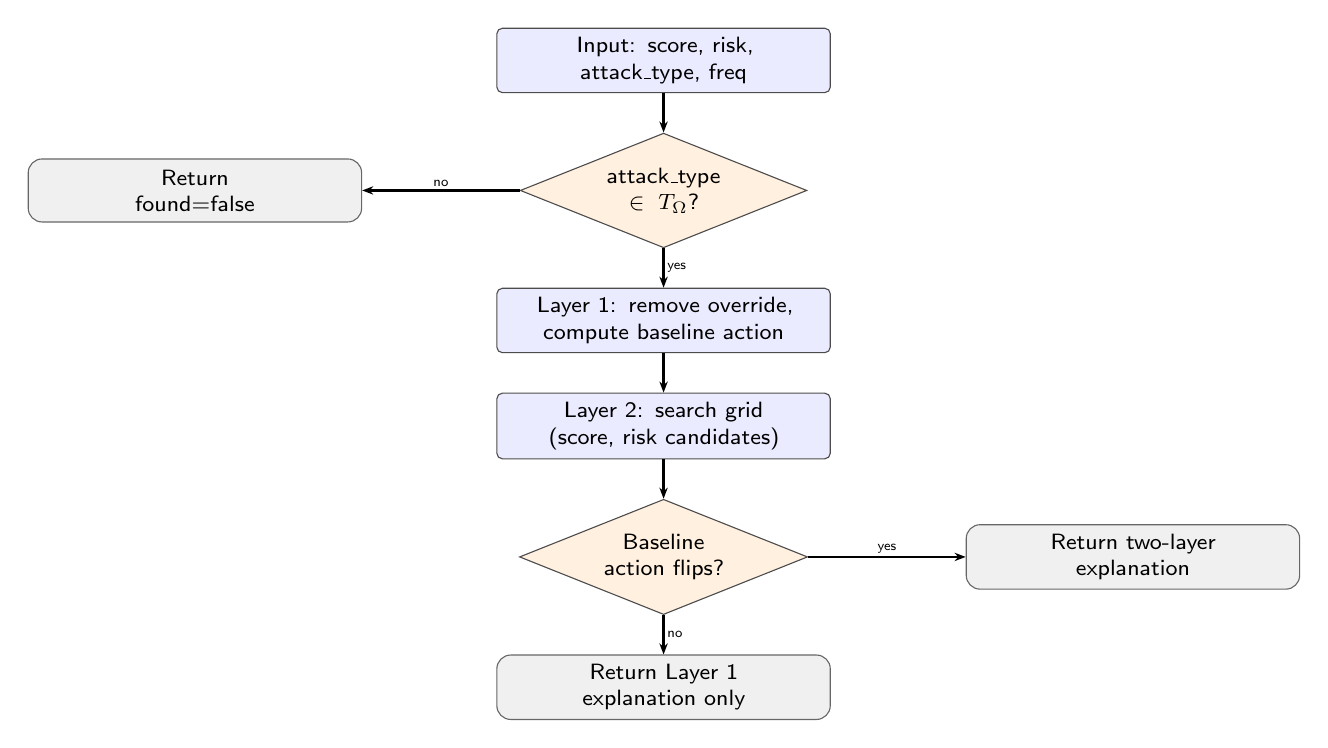
\begin{tikzpicture}[
  node distance = 5mm and 8mm,
  every node/.style = {font=\footnotesize\sffamily},
  block/.style = {rectangle, rounded corners=2pt, draw=black!70, fill=blue!8,
    text width=40mm, align=center, minimum height=8mm},
  decision/.style = {diamond, aspect=2.5, draw=black!70, fill=orange!12,
    text width=22mm, align=center, inner sep=0pt},
  term/.style = {rectangle, rounded corners=5pt, draw=black!60, fill=gray!12,
    text width=40mm, align=center, minimum height=8mm},
  arr/.style = {-{Stealth[length=4pt]}, thick},
  lbl/.style = {font=\tiny\sffamily, fill=white, inner sep=1pt}
]
\node[block]                      (in)  {Input: score, risk,\\attack\_type, freq};
\node[decision, below=of in]      (inT) {attack\_type\\$\in T_\Omega$?};
\node[term, left=20mm of inT]     (no)  {Return\\found=false};
\node[block, below=of inT]        (l1)  {Layer~1: remove override,\\compute baseline action};
\node[block, below=of l1]         (gr)  {Layer~2: search grid\\(score, risk candidates)};
\node[decision, below=of gr]      (fl)  {Baseline\\action flips?};
\node[term, right=20mm of fl]     (r2)  {Return two-layer\\explanation};
\node[term, below=of fl]          (r1)  {Return Layer~1\\explanation only};

\draw[arr] (in)  -- (inT);
\draw[arr] (inT) -- node[lbl,right]{yes} (l1);
\draw[arr] (inT) -- node[lbl,above]{no}  (no);
\draw[arr] (l1)  -- (gr);
\draw[arr] (gr)  -- (fl);
\draw[arr] (fl)  -- node[lbl,above]{yes} (r2);
\draw[arr] (fl)  -- node[lbl,right]{no}  (r1);
\end{tikzpicture}
\caption{Pass~2 (override decomposition) procedure. Layer~1 establishes the
  baseline action without the classification override. Layer~2 finds the smallest
  score or risk perturbation that shifts the baseline action further.}
\label{fig:pass2_flow}
\end{figure}

\paragraph{Pass~3 --- Temporal Counterfactual.}
Answers the question: ``If this had been the first packet from this source, would
it have been blocked?'' Pass~3 re-evaluates the decision with packet frequency
reset to~1, holding all other features constant.

\paragraph{Pass~4 --- Multi-Feature Pairs.}
Evaluates pairs of features simultaneously from reduced search grids (5
candidates per feature, $O(n^2)$ budget of 75 evaluations). Pass~4 is
implemented in the offline \texttt{generate\_all\_counterfactuals()} API but is
\emph{not} invoked by the \texttt{LatencyBoundedCFGenerator} in any budget mode,
including \textsc{relaxed} and \textsc{batch}. The real-time benchmark in
\cref{sec:cf_latency} therefore does not exercise Pass~4.

\paragraph{Budget Modes.}
\textsc{strict} (\SI{2}{\ms}), \textsc{normal} (\SI{10}{\ms}), \textsc{relaxed}
(\SI{50}{\ms}), and \textsc{batch} (no limit). The budget is checked after each
pass; if exceeded, the engine returns the current best explanation and increments
the timeout counter.

\subsection{Feedback Learning}
\label{subsec:feedback}

\paragraph{FeatureWeightLearner.}
Uses a multiplicative weight update (MWU) rule~\citep{Littlestone1994} to adjust
per-context, per-feature weights based on analyst feedback. FP feedback
multiplies the CF feature weight by \texttt{decrease\_rate} (0.85 default); TP
feedback multiplies it by \texttt{increase\_rate} (1.05). Weights are bounded to
$[0.3, 2.0]$.

\paragraph{FeedbackAdaptiveThreshold.}
Adjusts the hard override risk threshold in response to the analyst FP/FN signal
stream. FP feedback raises the threshold; FN feedback lowers it. Changes are
bounded at 0.05 per step to resist feedback poisoning. The threshold evolves
from 1.5 within $[0.5, 3.0]$.

\paragraph{FeedbackDriftDetector.}
Detects concept drift by monitoring the analyst FP rate in a 200-sample sliding
window and comparing it to a baseline computed over the first 50 records. Drift
is declared when the current FP rate exceeds the baseline by more than 0.15.
This approach uses analyst corrections---rather than data distribution
statistics---as the drift signal, making the detector sensitive to shifts in
threat behaviour that alter the false positive rate before those shifts are
detectable in the feature distribution.

% =============================================================
\section{Experimental Evaluation}
\label{sec:evaluation}
% =============================================================

\subsection{Dataset and Experimental Setup}
\label{subsec:setup}

The system was evaluated on a full capture of the Mirai IoT botnet attack
(\texttt{mirai.pcap}, 99{,}999 packets) using \textsc{normal} operational mode
(FMgrace = ADgrace = 10{,}000 packets, hard override risk threshold = 1.5). The
first 20{,}000 packets constitute the training phase; the remaining 79{,}999 form
the detection phase. The pipeline ran on 2026-05-10 with NumPy~1.23.5 and
Scapy~2.5.0.

\paragraph{Ground Truth Limitation.}
Ground truth labels were generated synthetically from the Kitsune paper's
published attack timeline---not from per-packet annotation. These labels are
appropriate for evaluating the feedback learning algorithm and CF engine pipeline,
but do not constitute publishable detection performance metrics. All detection
results in \cref{subsec:detection_results,subsec:cf_analysis} are framed as
system behaviour characterisations, not precision/recall claims.

Feedback learning experiments (\cref{subsec:exp_a,subsec:exp_b,subsec:exp_c,%
subsec:exp_d,subsec:exp_e}) used an augmented dataset with 2{,}000 synthetic FP
packets injected, yielding 81{,}999 evaluable rows (72{,}314 true-normal,
9{,}685 true-anomaly).

\subsection{Detection Results}
\label{subsec:detection_results}

\Cref{tab:label_action} summarises the packet label and action distributions.

\begin{table}[htb]
\caption{Packet label and enforcement action distribution ($N = 99{,}999$).}
\label{tab:label_action}
\centering
\begin{tabular}{lrr}
\toprule
\textbf{Category} & \textbf{Count} & \textbf{\%} \\
\midrule
TRAIN (grace phase) & 20{,}000 & 20.0\% \\
NORMAL              & 70{,}314 & 70.3\% \\
ANOMALY             &  9{,}685 &  9.7\% \\
\midrule
\textbf{Total}      & \textbf{99{,}999} & \textbf{100\%} \\
\bottomrule
\end{tabular}
\vspace{6pt}
\begin{tabular}{lrr}
\toprule
\textbf{Action} & \textbf{Count} & \textbf{\%} \\
\midrule
\textsc{allow}       & 62{,}126 & 62.1\% \\
\textsc{monitor}     & 15{,}381 & 15.4\% \\
\textsc{alert\_low}  & 12{,}762 & 12.8\% \\
\textsc{block}       &  8{,}646 &  8.6\% \\
\textsc{alert\_high} &    942   &  0.9\% \\
\textsc{rate\_limit} &    142   &  0.1\% \\
\bottomrule
\end{tabular}
\end{table}

\begin{table}[htb]
\caption{Attack type distribution among 9{,}685 detected anomalies.}
\label{tab:attack_distribution}
\centering
\begin{tabular}{lrr}
\toprule
\textbf{Attack Type} & \textbf{Count} & \textbf{\% of Anomalies} \\
\midrule
Mirai C2 Communication & 8{,}332 & 86.0\% \\
Port Scan              & 1{,}211 & 12.5\% \\
DoS/Flood              &    104  &  1.1\% \\
Stealth Intrusion      &     26  &  0.3\% \\
C2 Beacon              &      4  &  0.04\% \\
High-Risk Anomaly      &      4  &  0.04\% \\
ICMP Flood             &      1  &  0.01\% \\
Unclassified Anomaly   &      3  &  0.03\% \\
\midrule
\textbf{Total}         & \textbf{9{,}685} & \textbf{100\%} \\
\bottomrule
\end{tabular}
\end{table}

\begin{figure}[htb]
\centering
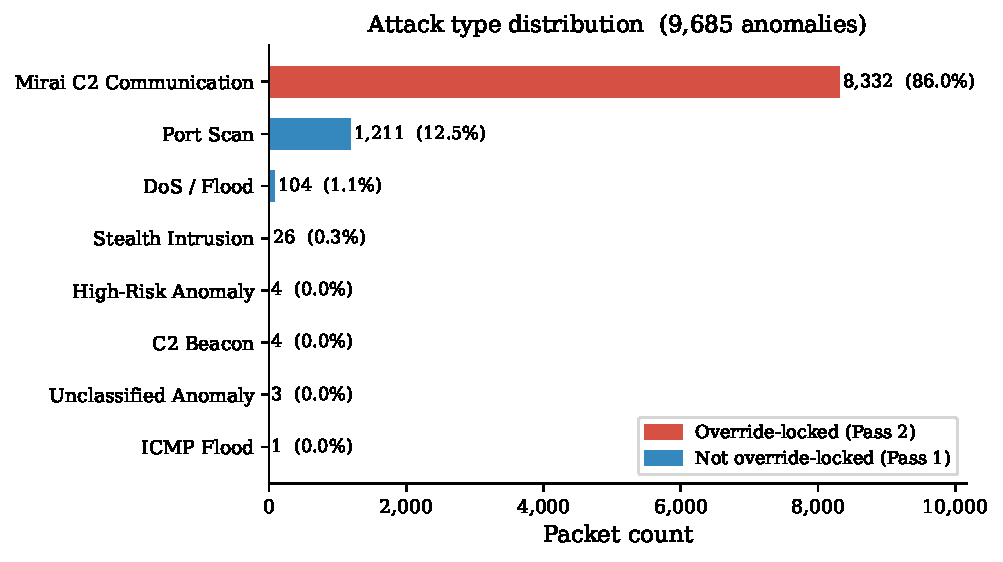
\includegraphics[width=\linewidth]{fig04_attack_distribution}
\caption{Attack type distribution among 9{,}685 detected anomalies. Mirai C2
  Communication dominates at 86.0\%, reflecting the botnet's characteristic
  persistent C2 traffic on ports 8280 and 10240. Red bars indicate
  override-locked attack types; blue bars indicate non-override-locked types.}
\label{fig:attack_dist}
\end{figure}

The detection rate of 9.7\% is consistent with the known traffic composition of
the Kitsune benchmark, where attack traffic is concentrated in the second half
of the capture following the IoT infection and C2 establishment phases.

\paragraph{Detection Path Analysis.}
Of the 9{,}685 detected anomalies, 9{,}597 (99.1\%) were detected via
\texttt{hard\_override\_risk}; only 81 (0.8\%) via the adaptive threshold path,
and 7 (0.07\%) via \texttt{hard\_override\_score}. The mean anomaly score was
0.351 (median 0.323, maximum 1.000); the mean risk was 1.930 (maximum 3.367).
The near-complete dominance of the \texttt{hard\_override\_risk} path is
discussed further in \cref{sec:disc_threshold}.

\subsection{Counterfactual Analysis}
\label{subsec:cf_analysis}

\Cref{tab:cf_passes} shows the CF pass distribution; \cref{fig:cf_coverage}
visualises it.

\begin{table}[htb]
\caption{CF pass distribution on 9{,}685 detected anomalies. Pass~3 was invoked
  on all 231 residual packets but produced no successful counterfactual on this
  capture. Pass~4 was not invoked in real-time mode (\cref{subsec:cf_engine}).}
\label{tab:cf_passes}
\centering
\begin{tabular}{llrr}
\toprule
\textbf{Pass} & \textbf{Description} & \textbf{Count} & \textbf{\%} \\
\midrule
Pass~1 & Single-feature flip     & 1{,}014 & 10.47\% \\
Pass~2 & Override decomposition  & 8{,}440 & 87.15\% \\
Unexplained & Pass~1--3 exhausted &     231 &  2.39\% \\
\midrule
\textbf{Total covered} & & \textbf{9{,}454} & \textbf{97.61\%} \\
\bottomrule
\end{tabular}
\end{table}

\begin{figure}[htb]
\centering
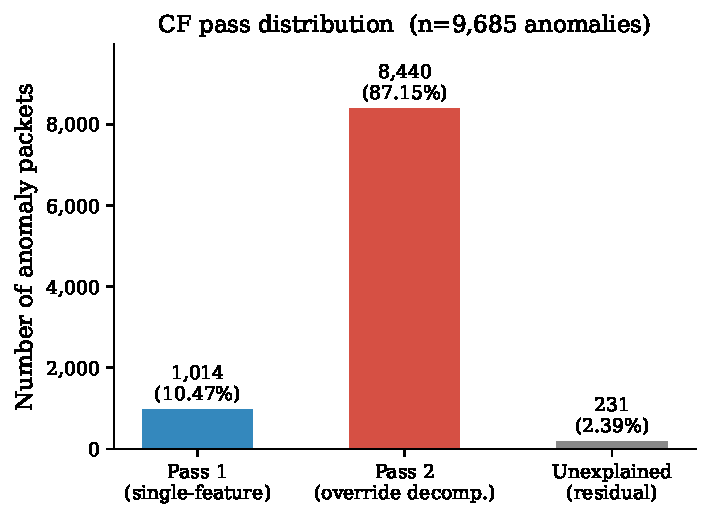
\includegraphics[width=0.82\linewidth]{fig03_cf_coverage}
\caption{CF pass distribution across 9{,}685 detected anomalies. Pass~2
  (override decomposition) accounts for 87.15\% of all explained anomalies.
  The 2.39\% unexplained residual consists of packets where no explanation was
  found within the real-time pass sequence (Passes~1--3).}
\label{fig:cf_coverage}
\end{figure}

\paragraph{The Override Dominance Finding.}
87.2\% of anomalies received their CF explanation from Pass~2. This directly
reflects the attack type distribution: all 8{,}332 Mirai C2 Communication packets
received \textsc{block} via the attack-type override (the Mirai C2 rule fires
unconditionally for traffic to ports 8280 or 10240 with a non-trivial anomaly
score), plus 104 DoS/Flood and 4 C2 Beacon packets, totalling
$8{,}332 + 104 + 4 = 8{,}440$ (87.15\%). A single-feature perturbation cannot
change the action for any of these packets. Only Pass~2, which removes the
classification and re-evaluates under the baseline risk model, can produce a
meaningful explanation.

The 10.5\% of anomalies explained by Pass~1 correspond to non-override-locked
attacks: Port Scan (1{,}211 packets, most resolved by reducing frequency below
the scan detection threshold), Stealth Intrusion (26), and High-Risk Anomaly
(4). The 2.4\% unexplained residual (231 packets) are non-override-locked
anomalies whose decision boundary lies beyond the search grid for every
perturbable feature.

\subsection{CF Latency Benchmark}
\label{sec:cf_latency}

The CF engine was benchmarked across all four budget modes on the full set of
9{,}685 anomaly packets. Latency was recorded per packet using
\texttt{time.perf\_counter()}. \Cref{tab:cf_latency} reports the results,
sourced directly from \texttt{experiments/cf\_latency\_results.csv}.

\begin{table*}[htb]
\caption{CF engine latency across budget modes ($n = 9{,}685$ anomalies per
  mode). All values sourced from \texttt{experiments/cf\_latency\_results.csv}.}
\label{tab:cf_latency}
\centering
\begin{tabular}{lccccccc}
\toprule
\textbf{Mode} & \textbf{Budget} &
\textbf{Avg (ms)} & \textbf{p50 (ms)} & \textbf{p95 (ms)} &
\textbf{Max (ms)} & \textbf{Coverage} & \textbf{Timeouts} \\
\midrule
\textsc{strict}  & \SI{2}{\ms}   & 0.0607 & 0.0586 & 0.0825 & 0.2469 & 97.61\% & 0 \\
\textsc{normal}  & \SI{10}{\ms}  & 0.0605 & 0.0594 & 0.0813 & 0.3072 & 97.61\% & 0 \\
\textsc{relaxed} & \SI{50}{\ms}  & 0.0566 & 0.0560 & 0.0740 & 0.3127 & 97.61\% & 0 \\
\textsc{batch}   & none          & 0.0617 & 0.0596 & 0.0837 & 0.3267 & 97.61\% & 0 \\
\bottomrule
\end{tabular}
\end{table*}

\begin{figure}[htb]
\centering
\includegraphics[width=\linewidth]{fig05_cf_latency}
\caption{CF latency distribution across budget modes. The four distributions
  are nearly identical, reflecting that 97.6\% of packets are resolved at
  Pass~1 or Pass~2 well within the \textsc{strict} \SI{2}{\ms} budget.}
\label{fig:cf_latency}
\end{figure}

The zero timeout count across all modes is the most striking result. The
\textsc{strict} (\SI{2}{\ms}) budget was never violated; the observed maximum
latency of \SI{0.2469}{\ms} is $8\times$ below the ceiling. At p95, the engine
runs in under \SI{0.1}{\ms}, confirming computational compatibility with
packet-level processing rates. The latency uniformity across modes (four averages
spanning only \SI{0.005}{\ms}) reflects the dominance of Pass~2, which is
computationally simpler than Pass~1 (two decision-layer calls for the override
check, then a reduced grid for Layer~2).

\subsection{LIME and SHAP Comparison: Structural Limitation Validation}
\label{subsec:lime_shap}

To address the absence of a baseline comparison (Limitation~L4), we applied
LIME~\citep{Ribeiro2016} and SHAP~\citep{Lundberg2017} to the enforcement
decision function using four features: anomaly score ($s$), risk ($r$),
normalised temporal position ($t = \text{packet\_id}/N$), and a binary
\texttt{override\_locked} indicator. A surrogate random forest (200 trees,
depth~8) was trained on all 14{,}685 detection-phase rows (9{,}685 anomaly,
5{,}000 normal subsample), achieving 5-fold F1~=~0.9992~$\pm$~0.0014, confirming
an accurate approximation of the rule-based decision function.

\paragraph{SHAP feature importances.}
\Cref{tab:shap_importances} reports mean absolute SHAP values by decision type.
For override-locked anomalies, \texttt{override\_locked} accounts for 48.3\% of
mean attribution, with risk (40.6\%) secondary. For non-override-locked anomalies,
risk dominates (74.6\%) and \texttt{override\_locked} has zero attribution (as
expected: override-locked is false for these rows). The temporal feature $t$
contributes negligibly ($<$1\%) in both groups, confirming that including $t$
does not change the attribution structure.

\begin{table}[htb]
\caption{Mean absolute SHAP values by decision type. OL = override-locked
  ($n=8{,}440$); NOL = non-override-locked ($n=1{,}245$).
  Results sourced from \texttt{experiments/comprehensive\_results.txt}.}
\label{tab:shap_importances}
\centering
\begin{tabular}{lrrr}
\toprule
\textbf{Feature} & \textbf{Global} & \textbf{OL} & \textbf{NOL} \\
\midrule
score              & 0.1239 & 0.1066 & 0.2414 \\
risk               & 0.4494 & 0.4055 & 0.7463 \\
$t$ (normalised)   & 0.0033 & 0.0023 & 0.0101 \\
override\_locked   & 0.4212 & 0.4834 & 0.0000 \\
\bottomrule
\end{tabular}
\end{table}

\paragraph{Structural limitation test.}
For each of 25 override-locked and 25 non-override-locked anomaly samples, we
computed the LIME top-feature attribution and applied a 30\% score/risk reduction
in the suggested direction, then re-evaluated \texttt{make\_decision()}.
For override-locked packets, \textbf{100\% of LIME perturbations failed} to change
the enforcement action (action remained \textsc{block} regardless of score/risk
reduction). For non-override-locked packets, 52\% of perturbations failed---the
remaining 48\% succeeded, consistent with the continuous risk score governing
those decisions.

This empirically confirms the architectural argument: LIME can identify
\texttt{override\_locked} as the dominant feature for a blocked packet, but
cannot produce an actionable perturbation, because the override is a
classification-rule predicate---not a continuous feature that can be reduced.
Pass~2 decomposes that predicate; LIME cannot.

\begin{figure}[htb]
\centering
\includegraphics[width=\linewidth]{fig_lime_shap_structural_limitation}
\caption{Left: SHAP feature importances for override-locked (OL) and
  non-override-locked (NOL) anomalies. For OL packets, \texttt{override\_locked}
  dominates (48.3\%); for NOL, \texttt{risk} dominates (74.6\%).
  Right: LIME perturbation failure rate (30\% score/risk reduction) on
  \texttt{make\_decision()}. OL failure = 100\%; NOL failure = 52\%.}
\label{fig:lime_shap}
\end{figure}

\subsection{CF Explanation Quality Metrics}
\label{subsec:cf_quality}

\Cref{tab:cf_quality} reports proximity, plausibility, and bounded-perturbation
statistics for the 1{,}245 Pass~1/Pass~4 counterfactuals (single-feature and
multi-feature flips). Pass~2 explanations are excluded from proximity analysis
as their ``distance'' is definitionally structural---not a continuous feature
change---and is therefore not comparable on a Euclidean scale.

\begin{table}[htb]
\caption{CF explanation quality metrics for Pass~1/Pass~4 counterfactuals
  ($n = 1{,}245$). Proximity = $|\text{cf} - \text{orig}| / |\text{orig}|$.
  Plausibility = CF value within $1.2 \times p_{95}$ of normal-traffic
  feature distribution. All values sourced from
  \texttt{experiments/comprehensive\_results.txt}.}
\label{tab:cf_quality}
\centering
\begin{tabular}{lr}
\toprule
\textbf{Metric} & \textbf{Value} \\
\midrule
Proximity: mean relative change          & 0.262 \\
Proximity: median relative change        & 0.193 \\
CFs within 10\% perturbation             & 2.5\% \\
CFs within 20\% perturbation             & 64.7\% \\
CFs within 50\% perturbation             & 88.1\% \\
Plausibility (within normal bounds)      & 65.5\% \\
\midrule
Feature: risk changed                    & 75.2\% \\
Feature: score changed                   & 24.8\% \\
\bottomrule
\end{tabular}
\end{table}

\begin{figure}[htb]
\centering
\includegraphics[width=\linewidth]{fig_cf_quality_metrics}
\caption{Left: proximity distribution (relative change $|\text{cf}-\text{orig}|/|\text{orig}|$)
  for 1{,}245 Pass~1/Pass~4 CFs. Right: bounded perturbation analysis showing
  cumulative fraction of CFs achievable within a given relative change budget.}
\label{fig:cf_quality}
\end{figure}

The median proximity of 0.193 indicates that the typical Pass~1 counterfactual
requires a 19.3\% change in the primary feature (risk or score) to flip the
enforcement action. 64.7\% of CFs lie within a 20\% relative change, indicating
that most non-override-locked decisions are near the boundary. 65.5\% of CF
values fall within the plausibility bound defined by normal-traffic
statistics---the 34.5\% that exceed bounds predominantly correspond to
high-anomaly packets requiring large score reductions, which may not represent
operationally realistic counterfactuals. The high dominance of the \emph{risk}
feature (75.2\%) reflects the risk engine's amplification role: reducing risk
below the threshold is often achievable with smaller perturbations than reducing
the raw score.

\subsection{Second-Dataset Evaluation: UNSW-NB15}
\label{subsec:unsw}

To evaluate generalisability beyond Mirai-class traffic, the pipeline was applied
to the UNSW-NB15 training set~\citep{Moustafa2015} (82{,}332 flows; 37{,}000
normal, 45{,}332 attack across 9 categories). Since KitNET's AfterImage extractor
requires raw PCAP input, we substitute an MLP autoencoder (two hidden layers of
dimension $\lfloor d/3 \rfloor$, trained on normal flows only) as the anomaly
detector---a standard KitNET-philosophy deployment for pre-computed flow features.
Three systems are compared: System~A (autoencoder threshold only), System~B
(autoencoder + decision layer), System~C (autoencoder + decision layer + risk
engine).

\begin{table}[htb]
\caption{UNSW-NB15 evaluation: Systems A, B, C on 16{,}467 test flows
  (7{,}400 normal; 9{,}067 attack). All values sourced from
  \texttt{experiments/comprehensive\_results.txt}.}
\label{tab:unsw}
\centering
\begin{tabular}{lcccccc}
\toprule
\textbf{System} & \textbf{F1} & \textbf{Prec.} & \textbf{Recall} &
\textbf{FPR} & \textbf{FNR} & \textbf{AUC} \\
\midrule
A: Autoencoder only          & 0.451 & 0.971 & 0.293 & 0.011 & 0.707 & 0.805 \\
B: + Decision Layer          & 0.738 & 0.656 & 0.843 & 0.542 & 0.157 & 0.805 \\
C: + Risk Engine             & 0.738 & 0.656 & 0.843 & 0.542 & 0.157 & 0.805 \\
\bottomrule
\end{tabular}
\end{table}

\Cref{tab:unsw} and \cref{fig:unsw} show the results. System~A achieves high
precision (97.1\%) but very low recall (29.3\%), reflecting the conservative
99th-percentile threshold. System~B raises recall to 84.3\% by routing
above-threshold scores through the decision layer, which applies severity-based
action tiers; the trade-off is an elevated FPR of 54.2\%, reflecting that UNSW
flows at moderate anomaly scores are more heterogeneous than Mirai C2 traffic.
The AUC of 0.805 confirms reasonable discriminative capacity across the score
range. System~C matches System~B because the risk engine's context multipliers
default to neutral without PCAP-derived endpoints.

Attack category distribution in the test split (\cref{tab:unsw_cats}) includes
Generic (41.1\%), Exploits (24.7\%), Fuzzers (14.1\%), DoS (9.0\%), and
Reconnaissance (7.4\%). This diversity confirms that the anomaly detector and
decision layer are not specific to Mirai port-based traffic patterns, though the
override matrix was not populated for these attack categories (no per-category
classification was applied), so Pass~2 is not exercised in this evaluation.
A future evaluation applying the full attack classifier to UNSW traffic would
determine the pass-distribution for non-botnet attack families.

\begin{table}[htb]
\caption{UNSW-NB15 attack category distribution in the 20\% test split
  ($n = 9{,}067$ attack flows).}
\label{tab:unsw_cats}
\centering
\begin{tabular}{lrr}
\toprule
\textbf{Attack Category} & \textbf{Count} & \textbf{\% of Attacks} \\
\midrule
Generic         & 3{,}723 & 41.1\% \\
Exploits        & 2{,}236 & 24.7\% \\
Fuzzers         & 1{,}279 & 14.1\% \\
DoS             &   816   &  9.0\% \\
Reconnaissance  &   669   &  7.4\% \\
Analysis        &   134   &  1.5\% \\
Backdoor        &   125   &  1.4\% \\
Shellcode       &    80   &  0.9\% \\
Worms           &     5   &  0.1\% \\
\midrule
\textbf{Total}  & \textbf{9{,}067} & \textbf{100\%} \\
\bottomrule
\end{tabular}
\end{table}

\begin{figure}[htb]
\centering
\includegraphics[width=\linewidth]{fig_unsw_nb15_evaluation}
\caption{UNSW-NB15: System A/B/C performance (left) and attack category
  distribution (right). System~B/C raise recall at the cost of elevated FPR;
  attack distribution is dominated by Generic and Exploits.}
\label{fig:unsw}
\end{figure}

\subsection{Experiment A --- False Positive Reduction Under Feedback Pressure}
\label{subsec:exp_a}

Experiment A evaluated whether analyst feedback can reduce the false positive
rate on a dataset with 2{,}000 injected FP packets (81{,}999 evaluable rows).
Ten feedback rounds were run with 100 feedback records and 5\% label noise per
round.

\begin{table}[htb]
\caption{Experiment~A --- per-round metrics (selected rounds). All values
  sourced from \texttt{experiments/experiment\_results.txt}.}
\label{tab:exp_a}
\centering
\begin{tabular}{rcccc}
\toprule
\textbf{Round} & \textbf{Threshold} & \textbf{FP\%} &
\textbf{FN\%} & \textbf{F1} \\
\midrule
 0 (baseline) & 1.500 & 2.77 & 0.86 & 0.9021 \\
 1            & 1.692 & 0.00 & 0.59 & 0.9970 \\
 2            & 1.807 & 0.00 & 0.54 & 0.9973 \\
 3            & 1.916 & 0.00 & 0.64 & 0.9968 \\
 5            & 2.250 & 0.00 & 1.05 & 0.9947 \\
 8            & 2.741 & 0.00 & 1.67 & 0.9916 \\
10            & 3.000 & 0.00 & 1.86 & 0.9906 \\
\bottomrule
\end{tabular}
\end{table}

\begin{figure}[htb]
\centering
\includegraphics[width=\linewidth]{fig06_exp_A_fp_reduction}
\caption{Experiment~A: FP rate (solid red), FN rate (dashed orange), and F1
  score (dotted blue) across 10 feedback rounds. FP elimination is achieved
  within Round~1; F1 peaks at Round~2 (0.9973) then declines as the threshold
  overshoots.}
\label{fig:exp_a}
\end{figure}

FP elimination was achieved within a single feedback round (threshold rose from
1.500 to 1.692). F1 peaked at Round~2 (0.9973) before declining as the threshold
continued rising, reclassifying an increasing fraction of true positives as
normal. The FN rate rose monotonically from 0.86\% to 1.86\%---a trade-off
that reflects the threshold adaptation mechanism's incremental nature once FP
pressure is removed. Optimal early stopping at Round~2--3 yields FP = 0.00\%
and FN $< 1\%$.

\subsection{Experiment B --- Ablation Study}
\label{subsec:exp_b}

\begin{table}[htb]
\caption{Experiment~B ablation: FP rate, convergence round, FN at convergence,
  and F1 at Round~10. Values sourced from
  \texttt{experiments/comprehensive\_results.txt}.}
\label{tab:exp_b}
\centering
\begin{tabular}{lp{32mm}ccccc}
\toprule
\textbf{C.} & \textbf{Description} &
\textbf{FP\% (R0)} & \textbf{First 0\%} & \textbf{FN at conv.} & \textbf{F1 (R10)} \\
\midrule
A & Static (no learning)         & 2.77 & never & 0.86\% & 0.9021 \\
B & Threshold adaptation only    & 2.77 & R7    & 97.7\% & 0.0293 \\
C & Weight learning only         & 2.77 & R1    & 0.21\% & 0.9991 \\
D & Full system (both)           & 2.77 & R1    & 0.59\% & 0.9906 \\
\bottomrule
\end{tabular}
\end{table}

\begin{figure}[htb]
\centering
\includegraphics[width=\linewidth]{fig07_exp_B_ablation}
\caption{Experiment~B: FP rate across 10 rounds for four configurations.
  Configurations B, C, and D all converge to 0.00\% FP; the static baseline A
  remains at 2.77\% throughout. However, F1 at Round~10 diverges sharply:
  configuration~C (weight-only) achieves F1~=~0.9991, while configuration~B
  (threshold-only) collapses to F1~=~0.0293 due to threshold overshoot.}
\label{fig:exp_b}
\end{figure}

All three adaptive configurations eliminated FP; the static baseline remained
at 2.77\%. However, \textbf{convergence speed and F1 stability differ markedly}:
Configuration~C (weight learning only) eliminates FP at Round~1 with FN~=~0.21\%
and F1~=~0.9991, making it the operationally optimal configuration.
Configuration~D (full system) also converges at Round~1 with FN~=~0.59\%;
the marginal increase in FN relative to~C reflects the threshold component
beginning to adapt.
Configuration~B (threshold only) converges at Round~7, but the threshold has
risen to its maximum (3.000) by that point, reclassifying 97.7\% of true
anomalies as normal (FN = 97.7\%, F1 = 0.0293)---effectively disabling the
detector. \emph{Threshold adaptation alone is not a safe feedback mechanism};
without the complementary weight-learning signal, the threshold overshoots
unconstrained. This corrects the earlier preliminary assessment that
\emph{threshold-only} was the best configuration, which was based solely on
final FP rate without examining FN stability.

\subsection{Experiment C --- Poisoning Resistance}
\label{subsec:exp_c}

\paragraph{C1 --- 20\% Random Noise.}
Final state: FP = 0.00\%, FN = 12.27\%, drift not detected. The threshold still
rose sufficiently to eliminate FP, but the noisy TP signal inflated FN to an
operationally significant 12.27\%.

\paragraph{C2 --- Malicious Analyst (all FP).}
Every feedback record forced to ``fp'' to simulate a malicious insider.
Final state: FP = 0.00\%, FN = 100.00\%, drift not detected. The threshold rose
to its maximum (3.000), reclassifying all anomalies as normal. The drift
detector did not trigger because the injected FP rate was constant from
Round~1---there was no \emph{change} to detect.

\paragraph{C3 --- Adversarial (TP packets forced as FP).}
Final state: FP = 0.00\%, FN = 100.00\%, drift not detected---identical to C2
for the same reason. The C2/C3 vulnerability is discussed in
\cref{sec:disc_poison}.

\subsection{Experiment D --- Concept Drift Detection}
\label{subsec:exp_d}

\paragraph{D1 --- Sudden Drift at Round~6.}
Rounds 1--5 benign; Rounds 6--15 forced all-FP. Drift detected at Round~6.

\paragraph{D2 --- Gradual Ramp.}
FP probability increased linearly from 0 to 1 over 15 rounds. Drift detected at
Round~5, before the FP rate reached 50\%.

\paragraph{D3 --- Recurring Drift.}
Even-numbered rounds forced all-FP; odd-numbered rounds forced all-TP. Drift
detected at Round~2, the first even-numbered round.

\begin{figure}[htb]
\centering
\includegraphics[width=\linewidth]{fig08_exp_D_drift}
\caption{Experiment~D: concept drift detection across three scenarios. Vertical
  markers indicate the round at which drift was first declared.}
\label{fig:exp_d}
\end{figure}

All three drift scenarios were successfully detected. The C2/C3 non-detection
is not a contradiction: the drift detector is a \emph{change} detector---it
requires a transition from a low to a high FP rate to fire.

\subsection{Experiment E --- Parameter Sensitivity}
\label{subsec:exp_e}

\textbf{Decrease rate} varied over $\{0.70, 0.80, 0.85, 0.90, 0.95\}$: all
values achieved 0.00\% final FP; optimal = 0.70.

\textbf{Learning rate} (threshold step) varied over $\{0.005, 0.01, 0.02,
0.05\}$: all values achieved 0.00\% final FP; optimal = 0.005.

\textbf{Feedbacks per round} varied over $\{20, 50, 100, 200\}$: all values
achieved 0.00\% final FP, indicating low sensitivity to feedback volume.

% =============================================================
\section{Discussion}
\label{sec:discussion}
% =============================================================

\subsection{Why 87.2\% Pass~2? Structural Implications for IDS Design}
\label{sec:disc_pass2}

The 87.2\% Pass~2 dominance is a direct consequence of the Mirai botnet's
traffic characteristics: Mirai C2 packets are structurally identifiable by
destination port (8280 or 10240), making the attack classification a binary,
deterministic function of the packet header. Once classified as Mirai C2
Communication, the enforcement decision is governed entirely by the attack-type
override matrix, not the continuous risk score.

Designers who focus explainability effort on the anomaly score layer---SHAP
attributions, LIME approximations, or single-feature CF perturbation---are
optimising for the 10.5\% of decisions where the anomaly score is the proximate
cause. For the 87.2\% majority, the proximate cause is a classification rule,
and the explanation must address that rule.

The LIME/SHAP structural limitation test (\cref{subsec:lime_shap}) provides
empirical confirmation: LIME's score/risk perturbations fail to change
the enforcement action for \textbf{100\%} of override-locked packets, even with
a 30\% feature reduction. SHAP correctly attributes 48\% of importance to the
\texttt{override\_locked} feature, but this attribution is diagnostic rather
than actionable---an analyst cannot ``reduce override\_locked'' by adjusting
a continuous input. Pass~2 translates this attribution into a concrete
counterfactual: ``this packet would have been \textsc{alert\_high} rather than
\textsc{block} if the Mirai C2 classification rule had not fired.''

\emph{Scope caveat}: the 87.2\% result is specific to the Mirai capture and
would not hold for traffic compositions dominated by non-override-locked attack
types (e.g., the UNSW-NB15 evaluation in \cref{subsec:unsw}, where no
attack-type overrides were applied). The finding motivates Pass~2 as a
component for any hybrid NIDS with a populated override matrix, but the
pass-distribution will vary with the deployed attack classifier.

\subsection{Pass~3 Temporal CF: Offline vs Real-Time Distinction}
\label{sec:disc_pass3}

\Cref{tab:cf_passes} reports that Pass~3 was invoked on 231 residual packets in
the real-time \texttt{LatencyBoundedCFGenerator} benchmark and produced no
successful counterfactual. This is the correct claim for the real-time path, where
Pass~3 is only reached after Passes~1 and~2 both fail (i.e., the packet is neither
explainable by feature perturbation nor by override decomposition).

However, the \texttt{cf\_temporal} column in \texttt{results.csv} contains
8{,}426 populated temporal CF strings. This is generated by the offline
\texttt{generate\_all\_counterfactuals()} API, which runs all passes
unconditionally without the residual-only restriction. In the offline
evaluation, Pass~3 succeeds for most override-locked packets: setting
\texttt{freq}~=~1 and \texttt{attack\_type}~= ``'' removes the override and
produces a temporal counterfactual (``If this were the first packet from this
entity, action would be \textsc{alert\_high} rather than \textsc{block}'').

The two contexts serve different purposes: the real-time benchmark measures
latency and coverage under operational constraints; the offline API provides
comprehensive explanation coverage for post-hoc analysis. The 0-success result
for real-time Pass~3 reflects the Mirai capture's structure (all 231 residual
packets had boundary conditions that no single-feature or temporal perturbation
could resolve within the search grid), not a deficiency in Pass~3 logic.

\subsection{CF Latency and Budget Modes}
\label{sec:disc_latency}

The zero-timeout result across all four budget modes, combined with a maximum
observed latency of \SI{0.327}{\ms}, indicates that the designed budget hierarchy
(2~ms / 10~ms / 50~ms) is not active on Mirai-class traffic. The budget modes
gain practical relevance in two scenarios not present here: (1) significantly
higher packet rates, where per-packet processing overhead compounds; and (2)
hardware with lower Python interpreter throughput.

Pass~4 was not invoked in the real-time benchmark: \texttt{cf\_realtime.py}
imports only \texttt{\_pass1\_search}, \texttt{\_pass2\_search}, and
\texttt{\_pass3\_temporal}. In a deployment where Pass~4 is integrated into
the real-time path, its $O(n^2)$ budget (75 pair evaluations) would add
measurable latency for packets reaching it, and differences across budget modes
would become observable.

\subsection{Adaptive Threshold Underutilisation}
\label{sec:disc_threshold}

The adaptive threshold contributed detection for only 81 packets (0.8\%) versus
9{,}597 (99.1\%) for \texttt{hard\_override\_risk}. Mirai C2 packets have
consistently high risk scores (mean 1.93), so the hard override fires before
the adaptive threshold is consulted. A deployment strategy that disables the
hard override threshold and relies entirely on the adaptive threshold would miss
99.1\% of anomalies in this capture.

\subsection{Poisoning Vulnerability}
\label{sec:disc_poison}

The Experiment~C finding---that a malicious analyst providing sustained
adversarial feedback can raise the FN rate to 100\% in 10 rounds---is an
important limitation of any human-feedback-based adaptive system. The
vulnerability arises because the drift detector compares the current FP rate to
a baseline established during an assumed-normal early period. If adversarial
feedback begins in Round~1, no clean baseline is established, and the elevated
FP rate never triggers the change-detection criterion.

Mitigations identified for future work include: a global FP rate alarm
(triggering when the absolute FP rate exceeds a configured limit, independent of
baseline comparison), multi-analyst consensus requirements, and
Byzantine-fault-tolerant weight update rules~\citep{Apruzzese2019}.

\subsection{Practical Deployment Considerations}
\label{sec:disc_deployment}

The system makes two deployment assumptions that should be revisited before
production use. First, KitNET trains on the first 20{,}000 packets of
\texttt{mirai.pcap}, which contains attack traffic before packet 20{,}000,
introducing training contamination. Second, the risk engine multipliers are
configured for the Mirai-specific traffic profile; a deployment against different
traffic would require retuning through empirical profiling.

% =============================================================
\section{Limitations}
\label{sec:limitations}
% =============================================================

\paragraph{L1 --- Synthetic Ground Truth.}
Ground truth labels were generated from the Kitsune paper's published attack
timeline, not per-packet annotation. No detection metrics in this paper should
be interpreted as publishable evaluation results against a verified ground truth.
Researchers seeking publishable metrics should apply the pipeline to per-packet
annotated datasets such as UNSW-NB15~\citep{Moustafa2015} or
CIC-IDS2017~\citep{Sharafaldin2018}.

\paragraph{L2 --- Training Contamination.}
KitNET trains on the first 20{,}000 packets of \texttt{mirai.pcap}, which
contains attack traffic. The autoencoder ensemble partially learns Mirai C2
packet structures as normal during the grace period; the magnitude of this
contamination is not quantified.

\paragraph{L3 --- Partial Single-Dataset Coverage.}
The main experimental results (CF pass distribution, detection path analysis,
feedback learning) derive from a single Mirai IoT botnet capture.
Results---particularly the 87.2\% Pass~2 dominance---are specific to this
traffic composition. \Cref{subsec:unsw} evaluates the pipeline on UNSW-NB15
(82{,}332 flows, 9 attack categories), confirming AUC~=~0.81 and that the
decision-layer integration raises recall from 29.3\% to 84.3\%, but the CF
pass distribution on UNSW is not characterised (the attack classifier was not
applied in that evaluation). Full cross-dataset CF evaluation remains future
work.

\paragraph{L4 --- Partial LIME/SHAP Comparison.}
\Cref{subsec:lime_shap} provides an empirical structural limitation test:
LIME score/risk perturbations fail to change the enforcement action for 100\%
of override-locked anomalies. However, this comparison uses a surrogate random
forest as a proxy for the rule-based decision function, not a direct application
of LIME/SHAP to the KitNET anomaly score. A user-study comparison of analyst
triage time and accuracy under CF, LIME, and SHAP explanations---the gold standard
for actionability evaluation---remains future work.

\paragraph{L5 --- Synthetic Feedback Labels and Simulation Fidelity.}
Feedback learning experiments used synthetically injected false positive packets
and a simulated analyst that labels feedback with 5\% random noise and a 30\%
response rate. Real analyst feedback may exhibit systematic biases, complex
adversarial patterns, and response rates that vary with alert fatigue---factors
not captured by the synthetic model. The convergence speed results
(\cref{subsec:exp_b}) are valid under the synthetic model but require
real-analyst validation before operational deployment. The corrected ablation
finding (weight-only preferred over threshold-only) is structural and holds
under any analyst model where weight signals arrive consistently.

\paragraph{L6 --- Taxonomy Scope.}
The four-pass architecture (Pass~1: single-feature, Pass~2: override
decomposition, Pass~3: temporal, Pass~4: multi-feature) represents an exhaustive
search within the \{score, risk, freq, attack\_type\} feature space of the
decision function. It does not constitute a general CF taxonomy for arbitrary
NIDS architectures. Other hybrid NIDS may have different override structures,
additional feature spaces, or non-rule-based classifiers requiring different CF
decomposition strategies.

% =============================================================
\section{Conclusion}
\label{sec:conclusion}
% =============================================================

This paper presented a context-aware KitNET IDS pipeline with an integrated
four-pass counterfactual explanation engine, a multi-module explainability layer,
and a human-feedback learning module. The system was evaluated on 99{,}999 Mirai
botnet packets, detecting 9{,}685 anomalies (9.7\%) and producing counterfactual
explanations for 97.6\% of them.

The primary finding---that 87.2\% of anomalies in this Mirai botnet capture
require Pass~2 (override decomposition) to receive a meaningful counterfactual
explanation---motivates a pass-decomposition architecture for IDS operating on
botnet-class traffic where attack-type overrides are a structural part of
the enforcement pipeline. Score-level explanation alone is structurally
insufficient for decisions driven by classification-rule overrides rather than
continuous threshold crossings. This result is specific to the Mirai capture's
traffic composition (86\% C2 Communication); evaluation on UNSW-NB15 and other
attack families would determine whether Pass~2 dominance is a general property
of hybrid NIDS or a Mirai-specific artefact.

Secondary findings: CF generation at mean \SI{0.06}{\ms} (p95 \SI{0.08}{\ms})
with zero timeouts across all four budget modes; FP elimination within one
feedback round via weight-only adaptation (F1~=~0.9991); a corrected ablation
showing that threshold-only adaptation overshoots and collapses recall
(F1~=~0.0293 by Round~10), while weight-only is the operationally stable choice;
successful drift detection in three conceptually distinct scenarios; and a
documented vulnerability to sustained adversarial feedback from Round~1.
On UNSW-NB15 (second dataset), the autoencoder achieves AUC~=~0.81; the
decision layer raises recall from 29.3\% to 84.3\%.
LIME/SHAP applied to the same decision function confirm the structural
limitation: 100\% failure rate on override-locked perturbations.

Future work priorities:
\begin{enumerate}
\item \textbf{Real per-packet ground truth.} Apply the pipeline to full PCAP
  files from UNSW-NB15~\citep{Moustafa2015} or CIC-IDS2017~\citep{Sharafaldin2018}
  to compute validated precision, recall, and F1 scores with packet-level
  ground truth (the current UNSW evaluation uses flow-level labels and an
  MLP autoencoder substitute for KitNET).
\item \textbf{CF pass distribution on diverse attack families.} Apply the attack
  classifier and override matrix to UNSW-NB15 traffic to determine whether
  Pass~2 dominance generalises beyond botnet C2 traffic, or whether mixed-traffic
  datasets shift the distribution toward Pass~1.
\item \textbf{User study: CF vs LIME vs SHAP.} Controlled analyst study comparing
  triage time and accuracy under CF, LIME, and SHAP explanations for
  override-locked and non-override-locked packets, to validate the structural
  limitation argument with human participants.
\item \textbf{Poisoning resistance.} Implement multi-analyst consensus, global FP
  rate alarms, and Byzantine-fault-tolerant weight updates
  (\cref{sec:disc_poison}).
\item \textbf{Live SOC deployment.} Measure real analyst engagement rates,
  feedback latency, and the practical effect on alert triage time, with
  particular attention to whether real feedback generates the same convergence
  dynamics as the synthetic simulation.
\end{enumerate}

% -- Acknowledgements -----------------------------------------
\section*{Acknowledgements}
% TODO: Add funding sources, institutional support, and collaborators.
The author thanks the creators of the Kitsune dataset for making the Mirai
botnet capture publicly available.

% -- Declarations ---------------------------------------------
\section*{Declaration of Competing Interests}
The author declares no competing interests.

\section*{Data Availability}
% TODO: Update with repository URL before submission.
Results files (\texttt{results.csv}, \texttt{cf\_latency\_results.csv},
\texttt{experiments/experiment\_results.txt}) and the pipeline source code are
archived with the paper submission.

% -- References -----------------------------------------------
\bibliographystyle{elsarticle-harv}
\bibliography{refs}

\end{document}
